\documentclass{article}
\usepackage[utf8]{inputenc}
\usepackage{tikz} 

\title{Graph Theory Notes Chapter 1}
\author{Sai Nallani}
\date{December 2022}

\begin{document}

\maketitle

\section{Graphs and Simple Graphs}
A graph G is a ordered triple $(V(G), E(G), \psi_G)$. Basically,
$V(G)$ is the set of vertices, $E(G)$ is the
set of edges, and $\psi_G(e)$ returns an unordered pair of
vertices given an edge.\\
Preferred Definition: A graph G has a set of vertices $E(G)$
and a set of unordered pairs of vertices called edges $V(G)$.\\
\subsection{Definitions}
Graphs that have a diagram whose edges intersect only at their ends are
called \textbf{planar}.
The graph below is \textbf{nonplanar} because edge $(v_3, v_6)$ intersects
with $(v_6, v_2)$ and $(v_2, v_5)$.\\
\begin{center}
    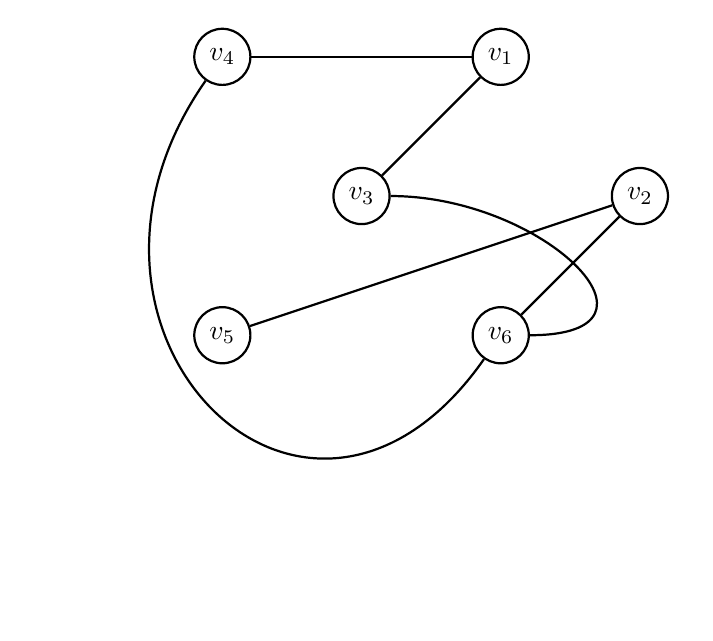
\begin{tikzpicture}[node distance={25mm},thick, main/.style = {draw, circle}]
        \node[main] (1) {$v_1$};
        \node[main] (2) [below right of=1]{$v_2$};
        \node[main] (3) [below left of=1]{$v_3$};
        \node[main] (4) [above left of=3]{$v_4$};
        \node[main] (5) [below left of=3]{$v_5$};
        \node[main] (6) [below left of=2]{$v_6$};
        \draw (2) -- (5);
        \draw (4) -- (1);
        \draw (4) to [out=235, in=235, looseness=2] (6);
        \draw (3) to (1);
        \draw (2) to (6);
        \draw (6) to [out=0, in=0, looseness=2] (3);
    \end{tikzpicture}\\
\end{center}
A vertex is \textbf{incident} with an edge if the vertex is an endpoint
of the edge (e.g. $v_1$ is incident with edge $(v_1, v_4)$). Two vertices,
$v_i$ and $v_j$, are adjacent if there exists an edge such that $(v_i, v_j)
\in E(G)$
\end{document}